\chapter{Introduction}

%%ASTRA
\section{What is ASTRA?}
\label{section:what-is-astra}
ASTRA (Awareness Services and Systems - Towards Theory and Realization)
\cite{astra02} is a project (logo in Figure \ref{img:astra-logo}) that
researches awareness systems and services that are used for social purposes. 
Awareness systems are computer-mediated communication systems that help
individuals or groups build and maintain a peripheral awareness of each other,
allowing them to stay in touch.

\begin{figure}
 \begin{center}
 
\includegraphics{img/astra_logo.png}
 \end{center}
 \caption{\label{img:astra-logo}ASTRA logo}
\end{figure}

Compared to telephony and video conferencing, awareness systems offer
low effort and non-intrusive communication throughout the day. The state of the
art is limited to non-functional prototypes without corresponding advances in
theory development. The assessment project aims to establish whether such systems
serve real and not imaginary user needs, through limited implementation and
testing. It will test social presence as the appropriate theoretical framework
for these systems and gain a first understanding of requirements for middleware
and interactive devices to support awareness services. ASTRA is a FET (Future and
Emerging Technologies) project under EU's Framework Programme 6 under contract
number IST-2001-39270, running in 2006-2009.

The organizations which are part of the ASTRA consortium are:

\begin{itemize}
  \item \verb|CTI| (Research Academic Computer Technology Institute), brings in
  experience in Designing Ambient Intelligence Systems (DAISy). 
  The CTI DAISy research team bridging computer science with interaction design will 
  lead the project and support with research in end user programming tools, design framework, 
  ontologies and modules development for the architecture.
  \item \verb|TU/e| (Industrial design), shall bring in expertise in interaction
  design, user interface technology and qualitative research methods for interaction design. 
  \verb|TU/e|, Technology Management, shall contribute expertise in quantitative methods for assessing 
  user experiences, social presence and experimental design. 
  \item \verb|Telenor|, shall bring in expertise on communication services and
  software architectures.
  \item \verb|Philips|, shall bring in experience in field studies and the
  design of user interfaces for entertainment and leisure. Philips will support user tests in realistic 
  conditions in the HomeLab, a simulated home-laboratory, especially built and equipped for 
  large scale field studies. 
  \item \verb|NTNU| (Norges Teknisk-Naturvitenskapelige Universitet), through
  Monica Divitini, professor of cooperation technologies in the Department of
  Information and Computer Science. This project has been developed as part of
  the work of this organization.
\end{itemize}

\section{ASTRA applications}
\label{subsec:intro-awareness-applications}
A key concept in the ASTRA project is an ASTRA application
\cite{astra-repo}. ASTRA applications represent the mean to transform the
services provided by the system into awareness applications. 
There are two different types of applications: ``Nimbus'' and ``Focus''
applications. Nimbus applications are used to make available 
awareness information to other users, while Focus applications are used to
decide what information we are interested in and in which way we want to 
receive that information.
Figure \ref{img:astra-applications-schema} shows a schema where we can see  the
relationship between the two types of application. In this case, the user 
Alice has decided to create an ASTRA Nimbus application to express her feelings 
(``thinking of you'') when she hugs a pillow. Once this application is
published  to certain community (``family'' in Figure 
\ref{img:astra-applications-schema}), the rest of the users that belong to  that
community can subscribe to it and define a way to receive the information by 
defining a Focus application. In the case of Figure 
\ref{img:astra-applications-schema}, Alice's brother has decided to visualize 
it using a lamp, which will be turned on when Alice's Nimbus application is
triggered. Therefore, the system has been able to capture and send
this awareness information in a taylorized way.

\begin{figure}[h!]
 \begin{center}
 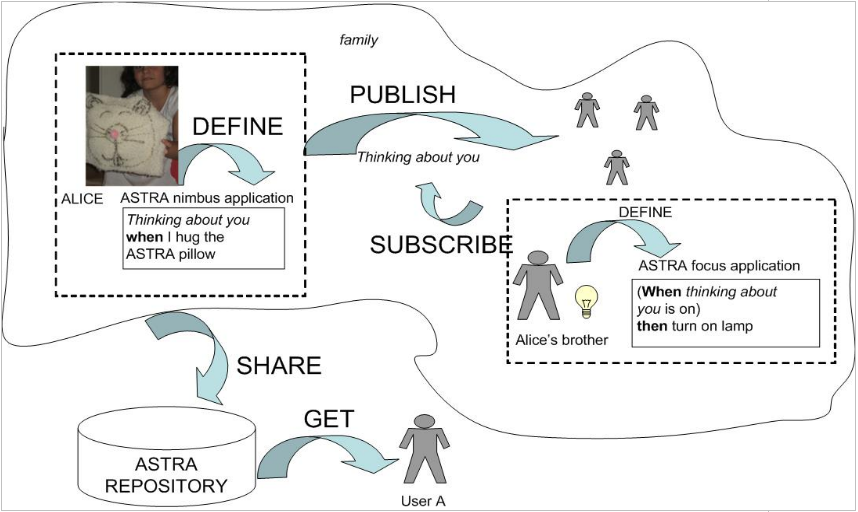
\includegraphics[scale=0.4]{screenshots/astra-applications-schema.png}
  \caption{\label{img:astra-applications-schema}ASTRA applications example}
 \end{center}
\end{figure}

\section{Motivations of the project}

The aim of this project is to create a system to manage the applications we
mentioned in Section \ref{subsec:intro-awareness-applications} and integrate
it into the ASTRA SOA (see Section \ref{subsubsec:tech-astra-soa}).
Managing comprises fuctionalities for sharing, tagging, locating,
appropriating and adapting the applications.
Figure \ref{img:astra-repository} shows the process of sharing and
appropriating applications through a central repository, illustrating the need
of customizing the parameters that are going to be shared (I.e.: for privacy
reasons) by user A, and the need of adapting the application to its
preferences (I.e.: connect it to his physical devices) by user B.
This process is potentially complex, therefore functionalities to help the user
to perform it are needed, as we will see in Section
\ref{subsec:implementation-app-adaptation}.
It is important to remark the difference between ``sharing'' and
``publishing''.  As we can see in Figure
\ref{img:astra-applications-schema}, sharing an application implies to upload a
taylorized set of information about it into the repository, but it does not
imply to send any kind of awareness information as in the case of publishing.
In the same way, ``retrieving"\footnote{We will use the verbs ``get'',
``appropriate'' or ``retrieve'' as synonyms when referring to an application in
this document.} an application from the repository implies to get it and taylorized
it, but not to subscribe to it.
On the other hand, once an user has appropriated and adapted the application, he
will be able to publish it as one made from the scratch.

\begin{figure}[h!]
 \begin{center}
 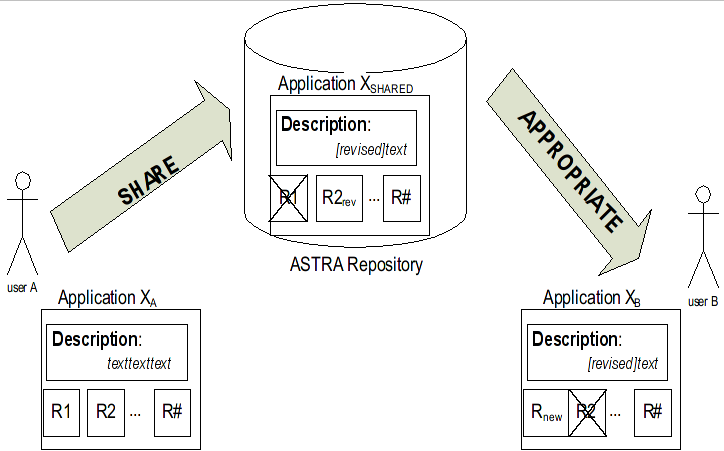
\includegraphics[scale=0.4]{screenshots/repository-appropiation.png}
  \caption{\label{img:astra-repository}Sharing and retrieving
  applications through the repository}
 \end{center}
\end{figure}

The rest of this document describes the process carried on to develop the
previously mentioned system, including a goals statement in Chapter
\ref{chap:objectives}, a explanation of the employed methodology and the
involved technologies in Chapter \ref{chap:methodology}, a detailed description
of the project in Chapter \ref{chap:description}, and a discussion of the
fulfillment of the goals and the personal contribution in Chapter
\ref{chap:conclusions}. 